\section{Signal \"ubertragungstrecke}
In diesem Versuch soll eine optische \"Ubertragunstrecke entworfen werden.
\subsection{Signalwandlung elektrisch-optisch}
In diesem Teil soll das elektrische Signal aus dem Signalgenerator mit Hilfe einer LED in ein optisches Signal umgewandelt werden.
\subsubsection{Experimentelle Durchf\"urung}
Es soll ein elektrisch-optischer Signalwandler aufgebaut werden, wie in Abbildung 5 zu sehen ist. An der LED m\"usste eine AC-Signal von ca. 90~$mV$ Amplitude messbar sein. Als Operationsverst\"arker wird NE5534 verwendet, da diese mehr Strom als TL082 treiben kann. Zwischen Pin 5 und Pin 8 des OPVs wird eine Kapazit\"at von C $=$ 680~$pF$ gesteckt werden. Die Kapazit\"at stabilisiert den OPV, um ungew\"unschte Schwingungen zu verhindern. In diesem Versuch werden folgende Widerst\"ande verwendet: 
\begin{eqnarray*}
R_1 &=& 9,1~k\Omega \\
R_2 = R_3 &=& 1~k\Omega \\
R_4 &=& 20~\Omega
\end{eqnarray*}
\begin{figure}[!h]
\begin{center}
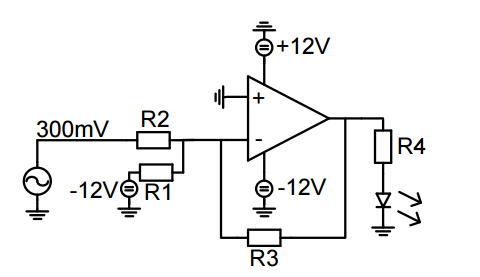
\includegraphics[scale=0.7]{bild/Signalwandler}
\caption{Invertierender Addierer zur elektrisch-optischen Signalwandlung}
\end{center}
\end{figure}
\subsubsection{Ergebnisse und Diskussion}
An der RL-LED wurde ein AC-Signal von ca. U$_{pp}$ $=$ 180~$mV$ gemessen, was eine Amplitude von ca. 90~$mV$ entspricht und somit unsere Schaltung verifiziert. Uns ist aufgefallen, dass die die Signalform am Ausgang kein reiner Sinus mehr ist. Dies l\"asst sich dadurch erkl\"aren, dass die RL-Diode die negative Signale schneidet. Das Schaubild wurde versehentlich gel\"oscht.  

\subsection{Signalwandlung optisch-elektrisch}
\subsubsection{Experimentelle Durchf\"uhrung}
Um die optische Dom\"ane in die elektrische r\"uckzuwandeln, wird ein Transimpedanzverst\"arker wie in Abbildung 6 zu sehen ist aufgebaut. Die Stromquelle I stellt hier die Photodiode dar, die das optische Signal von der IR-Diode in einen Strom umwandelt. Um eine gute Signal\"ubertragung zu erzeugen, sollten sich die beiden Dioden ber\"uhren.   
\begin{figure}[!h]
\begin{center}
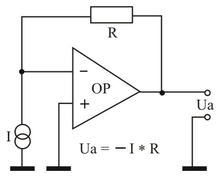
\includegraphics[scale=0.7]{bild/Transimpedanz}
\caption{Transimpedanzverst\"arker}
\end{center}
\end{figure}
\subsubsection{Ergebnisse und Diskussion}
Der Widerstand R des Transimpedanzverst\"arkers l\"asst sich durch die Formel, die in Abbildung 6 zu sehen ist, berechnen. In unserem Fall bei I $=$ 12,5~$\mu A$ betrug R $=$ 2~$k\Omega$, und dies hat ein Ausgangssignal von ca. 25~$mV$($\pm$ 20\%) Amplitude zur Folge. Das Ausgangssignal der Transimpedanzverst\"arkers ist in Abbildung 7 dargestellt.
\begin{figure}[!h]
\begin{center}
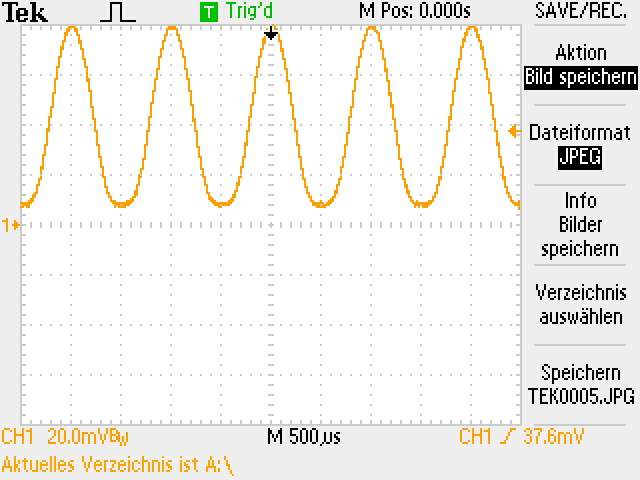
\includegraphics[scale=0.4]{bild/transimpedanzsignal}
\caption{Ausgang Transimpedanzverst\"arker}
\end{center}
\end{figure}
\subsection{Signalverst\"arkung uns Signalausgabe}
\subsubsection{Experimentelle Durchf\"uhrung}
Da die Signalamplitude von 25 mV  am Ausgang des Transimpedanzverst\"arkers nur ein leises Ton ausliefern kann, 
wird dessen Ausgang, um einen \textbf{TL082} Signalverst\"arker  erweitert. Dies soll des Spannung auf 1~$V$ erhoben, was ein Verst\"arkung von A $=$ 40 entspricht. Die Verst\"arkung wird durch folgende Formel bestimmt:
\begin{equation}
A = 1 + \frac{R_2}{R_1}
\end{equation}
\begin{figure}[!h]
\begin{center}
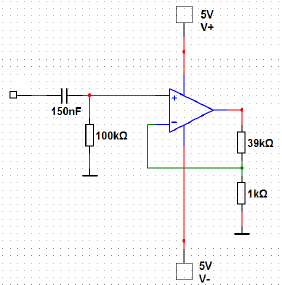
\includegraphics[scale=0.7]{bild/verstaerker40}
\caption{Operationsverst\"arker A = 40}
\end{center}
\end{figure}
Um eine Verst\"arkung von A = 40 zu erreichen, soll ein Verh\"altnis R$_1$ zu R$_2$ von 1 zu 39 sein. In unserem Fall wurden die Widerst\"ande wie folgt dimensioniert: 
\begin{eqnarray*}
R_1 &=& 1~k\Omega \\
R_2 &=& 39~k\Omega
\end{eqnarray*}
Um eine Offsetspannung zu vermeiden und zu entkoppeln, wird eine Kapazit\"at C~$=$~150~$nF$ und ein Widerstand R $=$ 100~$k\Omega$ als Hochpassfilter am Eingang aufgebaut. \\
Zun\"achst wurde ein Spannungsfolger, der mit Hilfe eines \textbf{NE5534} Operationsverst\"arkers aufgebaut ist, an den Ausgang des OPVs A = 40 verschaltet.\\
Schlie\ss lich werden zwei 1~$\mu F$ Gl\"attungkondensator zwischen positiver bzw. negativer Versorgungsspannung und Masse gesteckt, um die Spannungseinbr\"uchen entgegen zu wirken.\\
% die diese entkoppeln sollen. Schlie\ss lich wird am Ausgang ein 
\subsubsection{Ergebnisse und Diskussion}
Nach dem die Schaltung mit der Schaltung in Abbildung 9 erweitert wurde, wurde die Ausgangssignal nochmal gemessen und in Abbildung 9 dargestellt. Es wird aufgefallen, dass die Offsetspannung durch das Einsetzen des Kondensators entkoppelt worden ist, wie erwartet.
\begin{figure}[!h]
\begin{center}
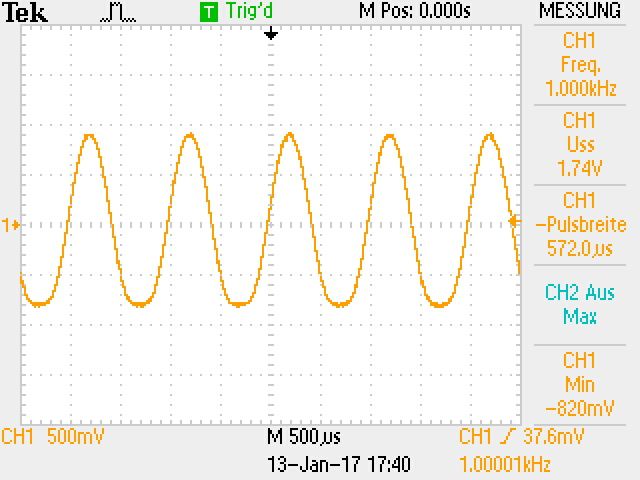
\includegraphics[scale=0.3]{bild/rc}
\caption{Signalausgabe des Operationsverst\"arker A = 40}
\end{center}
\end{figure}
Zun\"achst wurde der Lautsprecher angeschlossen, dabei ist kein starkes Ton zu h\"oren. Dies kann dadurch erkl\"aret werden, dass  der Lautsprecher einen h\"ohen Strom ben\"otigt, was dazu f\"uhrt, dass die Spannung am OPV zusammen bricht. \\
Um dies Effekt zu vermeiden, wurde mit einem Spannungsfolger erweitert.
Nach dem die genannten Schaltungen zusammen verschalten sind, konnte der Lautsprecher betrieben und Musik mit h\"ohreren Lautst\"arke gespielt werden.